\chapter{Phonemized CHILDES: A Phonemic Multi-Lingual Corpus of Child-Directed Speech}

\begin{roughdraft}
    The first content chapter of the thesis. Motivated by the need to have good quality multi-lingual phonemic datasets to do child acquisition experiments, it covers the following:
    \begin{itemize}[label=--]
        \item Motivation for using automated transcription tools to create phonemic datasets for language modeling (possibly covered in introduction). Movitation for having one multi-lingual dataset with a unified IPA format.
        \item Specific background related to datasets that exist (possibly covered in background chapter) and transcription tools that exist. Discuss the challenges behind creating phonemized datasets, the issues with IPA and previous approaches.
        \item Description of the Corpus Phonemizer tool, how it works and what it can do.
        \item The use of Corpus Phonemizer to produce Phonemized CHILDES. Describe Phonemized CHILDES dataset and what choices were made. 
        \item Corpus Analysis of Phonemized CHILDES across a wide range of experiments. 
    \end{itemize}
\end{roughdraft}

\section{Introduction and Background}
\label{sec:dataset-intro}

\rough{Specific background related to datasets that exist (possibly covered in background chapter) and transcription tools that exist. Discuss the challenges behind creating phonemized datasets, the issues with IPA and previous approaches. Explain the phonemic stream representation I want the datasets to have (space-separated phonemes with boundary markers).}

\section{Corpus Phonemizer}
\label{sec:dataset-corpus-phonemizer}

In order to address the challenges of automatically converting orthographic datasets to phonemic streams, I developed \corpusphonemizer,\footnote{\url{https://github.com/codebyzeb/Corpus-Phonemicizers}} a suite of tools and scripts for converting corpora into datasets using a consistent phoneme stream representation.

The primary tool in the suite is a command-line application \texttt{corpus\_phonemizer.py} which takes orthographic text as input and converts it to a unified phonemic representation in IPA. The tool supports many languages by leveraging backend transliteration tools which can be selected by the user, each of which provides a different set of language codes (see \cref{sec:dataset-transliteration-tool-backends}).

A crucial component of the tool is the use of \emph{folding dictionaries} to ensure that the set of phonemes produced by the backend transliteration tool for a particular language matches a standard phonemic inventory for that language. This validation step is important, \todo{expand on this}. It is also important to ensure that when designing the folding dictionaries, a consistent methodology is used. In order to support my multi-lingual experiments, I created folding dictionaries for 31 language codes. This process is described in \cref{sec:dataset-folding}.

The tool is versatile, supporting many options for ease-of-use when preparing corpora. Despite the tool's utility, there are still limitations to using an automated tool for creating phonemic transcriptions from orthographic text. I give example usage and discuss these limitations further in \cref{sec:dataset-usage,sec:dataset-limitations}.

Besides the command-line application, the \corpusphonemizer suite also contains scripts dedicated to preparing the specific datasets used in this thesis. These include:
\begin{itemize}
    \item The Phonemized CHILDES dataset 
    \item The BabyLM pre-training dataset
    \item The BLiMP, BLiMP Supplement and GLUE evaluation sets
    \item The British National Corpus (BNC)
\end{itemize}
Phonemized CHILDES is a large corpus of child-directed speech across 31 languages. I describe the creation of this dataset in \cref{sec:dataset-phonemized-childes}. The other datasets are in English and follow a similar process so I do not go into detail on their creation.

\subsection{Transliteration tool backends}
\label{sec:dataset-transliteration-tool-backends}

In order to convert orthographic text to phonemes, I leverage four transliteration tools, each of which supports a different set of languages. The tools use different approaches for different languages, including rule-based transliteration and dictionary pronunciations. In order to ensure a consistent output, I create a custom wrapper for each tool.

\paragraph{\texttt{phonemizer}:}
Phonemizer \citep{Bernard2021} is a python library that supports the automatic phonemization of text in many languages. It allows the user to select from one of four backends, each of which have different capabilities. By default, I use eSpeak \citep{Dunn2019}, an open-source speech synthesizer which supports over one hundred languages and outputs phonemes in IPA. This synthesizer uses a combination of handwritten rules and pronunciation dictionaries for each language it supports. Besides supporting many languages, it also supports many accents (such as Scottish English or Lancaster English) but only for a few languages besides English. For Japanese text written in Romanji, I instead use \texttt{phonemizer} with the Segments \citep{robert_forkel_2019_3549784} backend, which uses simple grapheme to phoneme mapping (Romanji has very simple pronunciation rules and is not supported by eSpeak).\footnote{\texttt{phonemizer}'s segments dictionary for Japanese was actually missing an entry to map `s' to /s/ but I was able to add this to their codebase and become a contributor of their project.}

\paragraph{\texttt{epitran}:}
Epitran \citep{Mortensen-et-al:2018} is similar to \texttt{phonemizer}, supporting the automatic phonemization of text across many languages with a particular focus on low-resource languages. For English it uses the Flite Speech Sythesis System \citep{black2001flite} as a backend and for Simplified and Traditional Chinese it uses the CC-CEDict dictionary\footnote{\url{https://cc-cedict.org}} but for the remaining 92 languages supported, it uses greedily-interpreted grapheme-to-phoneme maps augmented with context-sensitive pre-processor and post-processor rewrite rules. These are implemented using CSV files to facilitate the addition of new languages. The tool also supports alternative scripts for certain languages, such as Pinyin for Mandarin.

\paragraph{\texttt{pinyin\_to\_ipa}:} pinyin-to-ipa \citep{taubert_2024_pinyin-to-ipa_2024} is a python library for converting Mandarin written in pinyin to IPA using a few contextual grapheme-to-phoneme maps. The phoneme inventory is based on the phonology of Mandarin as described by \cite{lin2007sounds} and \cite{duanmu2007phonology} and tone markers are attached to the vowel of the syllable, rather than the end of the syllable. The tool only converts individual pinyin syllables, so my wrapper first splits the input into syllables (carefully maintaining word boundaries) before using the tool to convert each syllable to IPA.

\paragraph{\texttt{pingyam}:} Pingyam\footnote{\url{https://github.com/kfcd/pingyam}} is a table storing the conversion relationships between the various romanization systems of Cantonese, based on data from the Open Cantonese Dictionary.\footnote{\url{https://www.kaifangcidian.com/han/yue/}} Since the table also contains IPA, my \texttt{pingyam} wrapper uses the table to convert from the Jyutping romanization scheme to IPA by splitting the input text into syllables, finding each syllable in the table and outputting the corresponding IPA transcription. The table places tone markers after the syllables, so I implemented a utility to move the tone marker to be attached to the vowel of the syllable instead.

\subsection{Phoneme inventory validation}
\label{sec:dataset-folding}

For a given backend tool and language code, Corpus Phonemizer will convert orthographic text into phonemes. The specific set of phonemes produced will be drawn from a vocabulary determined by the specific rules or pronunciation dictionaries created for that backend and language code. Since these tools are open-sourced, and since the exact \textbf{phoneme inventory} of languages are often up for debate, it is important to ensure that the phoneme inventory produced by the backend-language choice is consistent with established phoneme inventories for that language.

For each backend-language pair used in this thesis, I examine the set of phonemes produced and compare them to the phoneme inventories for that language in \phoible, a database containing phoneme inventories extracted from source documents and tertiary databases for 2186 distinct languages \citep{phoible}. The database also contains phonetic feature information for each phoneme which is useful for comparing phonemes within an inventory. As there are often multiple inventories in \phoible for each language, I find the inventory that best matches the output phoneme set according to the number of phoneme types, the number of consonants, the number of vowels and the number of diphthongs.

Once the best inventory has been found, I use a process called \emph{folding} to align the output phoneme set with the inventory and correct errors in the output. Folding involves the construction of a look-up table (a \textbf{folding map}) which is applied to the output of the backend transliteration tool. There are several error types that can be solved using the folding map in order to align the phoneme sets, as detailed in \cref{tab:transcription-errors}. The most common of these are \textbf{one-to-one} errors, instances where the backend transliteration tool outputs a particular Unicode string for a specific phoneme but the inventory lists a different string, and so a simple one-to-one mapping can correct this. For example, the \texttt{phonemizer} backend with the \texttt{ja} language code (Japanese) outputs the tied characters \ttipa{\|c{ts}} as one of the phonemes, but the Japanese inventory we match with uses \ttipa{ts} instead. Another example is given in the top row of \cref{tab:transcription-errors}. These mappings that do not change the information-theoretic properties of the output (since the character(s) we map to do not already exist in the output) and only serve to match the symbols used in the inventory so that their phonetic features stored in \phoible can be used in further analyses.

\begin{table}[t]
    \centering
    \scriptsize
    \begin{tabular}{p{0.32\textwidth}p{0.26\textwidth}p{0.32\textwidth}}
    \toprule
        \textbf{Error type} & \textbf{Consequence} & \textbf{Example} \\
        \midrule
        \textbf{One-to-one:} The backend uses one symbol for a phoneme but the inventory lists a different symbol for that phoneme. & The one-to-one mapping does not change the number of types or tokens in the output. & \texttt{phonemizer} with language code \texttt{sv} (Swedish) outputs \ttipa{n} but the matching inventory uses \ttipa{\|[n}.\\
        \midrule
        \textbf{Many-to-one:} The backend produces two different phonemes that should only map to a single phoneme in the inventory. & The many-to-one mapping reduces the number of phoneme types. & \texttt{phonemizer} with language code \texttt{pt} (Portuguese) outputs both \ttipa{\*r} and \ttipa{r} but the matching inventory only lists \ttipa{K}.\\
        \midrule
        \textbf{Consonant merging:} The backend outputs two symbols for a consonant that should be written as a single phoneme. & The mapping merges the pair of consonants, reducing the number of phoneme tokens produced. & \texttt{epitran} with language code \texttt{srp-Latn} (Serbian) outputs the sequence \ttipa{d Z} but these are should be written as a single phoneme \ttipa{dZ}.\\
        \midrule
        \textbf{Vowel merging:} The backend outputs a pair of vowels as separate phonemes but they are typically analysed as a single diphthong. & The mapping merges the pair of vowels, reducing the number of phoneme tokens produced. & \texttt{pingyam} with language code \texttt{cantonese} outputs the sequence \ttipa{o u} but these are should be treated as a diphthong \ttipa{ou}.\\
        \midrule
        \textbf{Vowel splitting:} The backend outputs a diphthong that is not listed in the inventory and should be split into individual phonemes. & The mapping splits the pair of vowels, increasing the number of phoneme tokens produced. & \texttt{phonemizer} with language code \texttt{en-us} (American English) outputs \ttipa{aIU} as a single phoneme but this should be \ttipa{aI U}.\\
        \midrule
        \textbf{Phoneme duplication:} The backend outputs duplicate phonemes to represent long vowels or consonants or because of an error. & The mapping replaces the pair of phonemes with just one, reducing the number of phoneme tokens. & \texttt{phonemizer} with language code \texttt{et} (Estonian) outputs \ttipa{d d} but should output the long consonant \ttipa{d:}.\\
        \midrule
        \textbf{Diacritic error:} The backend incorrectly outputs the diacritic as a separate symbol instead of attaching it to the phoneme. & The mapping may change the number of phoneme types or tokens. & \texttt{phonemizer} with language code \texttt{ko} (Korean) outputs the diacritic for aspiration as \ttipa{h} instead of \ttipa{\super{h}} so sequences \ttipa{kh} and \ttipa{ph} are mapped to \ttipa{k\super{h}} and \ttipa{p\super{h}}.\\
        \midrule
        \textbf{Orthographic error:} Due to an invalid symbol in the orthographic text, the backend outputs an incorrect phoneme. & The contextual mapping changes the frequency statistics for the resulting phoneme, possibly reducing the number of phoneme types. & \texttt{epitran} with language code \texttt{hun-Latn} (Hungarian) outputs \ttipa{\^o} when the orthographic letter \textipa{\H{o}} is incorrectly written as \textipa{\^o} and so the phoneme is mapped to \ttipa{\o:}.\\
        \bottomrule
    \end{tabular}
    \caption{A list of errors that can occur during phonemization that can be fixed with a folding map but that may change the information-theoretic properties of the output.}
    \label{tab:transcription-errors}
\end{table}

The rest of the error types listed in \cref{tab:transcription-errors} are solved with mappings that are not necessarily one-to-one. These mappings may alter the number of output tokens or types by using a many-to-one mapping or by merging or splitting tokens. Since such a mapping will change the information-theoretic properties of the output, it is important that the they are linguistically motivated and carefully implemented. 

\subsubsection*{Folding map construction}

In order to construct the folding map for each backend-language pair, I run \corpusphonemizer on orthographic text for that language and compare the output set of phonemes $P_O$ to the phonemes in the closest inventory in \phoible $P_I$. I call the set of phonemes present in $P_O$ but not $P_I$ the ``unknown phonemes'' $U_K$ where $U_K = P_O \setminus P_I $ and the set of phonemes present in $P_I$ but not $P_O$ the ``unseen phonemes'' $U_S$ where $U_S = P_I \setminus P_O $. I then construct the folding map as follows:
\begin{enumerate}
    \item Find pairs $(k,s) \in U_K \times U_S$ that differ according to an accent or diacritic and obviously represent the same phoneme (determined by ruling out alternatives or examining where $k$ is produced in the output). Create a one-to-one mapping $k:s$ for each such pair, e.g. \ttipa{t} : \ttipa{t\super{h}}.
    \item Find pairs $(k,s) \in U_K \times U_S$ that clearly represent the same phoneme (determined as above) but may use entirely different symbols, possibly due to an alternative transcription scheme. Create a one-to-one mapping for each pair, e.g. \ttipa{a} : \ttipa{\ae}.
    \item For remaining items $k \in U_K$, determine whether these result from one of the other errors in \cref{tab:transcription-errors}. Carefully examine instances where $k$ is produced in the output and create a suitable mapping $k : p$ for some $p \in P_I$ to solve the error (the mapping may need to be contextual or include several characters, e.g. \ttipa{\textrhookschwa} : \ttipa{@ \*r} or \ttipa{U O} : \ttipa{w O}). 
    \item For remaining items $s \in U_S$, determine whether these result from one of the other errors in \cref{tab:transcription-errors}. Carefully examine instances where $s$ should be produced in the output and create a suitable mapping $k : s$ for some $k \in P_O$ to solve the error (the mapping may need to be contextual or include several characters). 
    \item Examine the output for cases of \textbf{phoneme duplication} and other errors that may not contain phonemes in $U_K$ or $U_S$ but could still be solved with the phoneme map and create suitable mappings.
\end{enumerate}

The goal is for $U_K = \{\} = U_S$ or equivalently $P_I = P_O$, i.e the set of phonemes produced by the tool perfectly aligns with the phoneme inventory in \phoible. This is not always possible, often there are a few remaining phonemes in $U_K$ and/or $U_S$. This can occur when no obvious mappings could be found in steps 1--4 above. For example, the \texttt{epitran} backend for German does not produce the phoneme \ttipa{Z} (it is ``unseen'') and none of the unknown phonemes seem to be a good match. Another possibility is that the output set of phonemes $P_O$ may not align well with any of the \phoible phoneme inventories and so the closest match may not include some of the unknown phonemes $k \in U_K$ despite being valid phonemes for that language and listed in other inventories. For example, the \texttt{epitran} backend for German produce the phonemes \ttipa{x} and \ttipa{5} which are not listed in the matching inventory but are listed in other established inventories for German. In other cases, the unknown phonemes may come from loan words (e.g. \ttipa{ts} for ``pizza'' in Portuguese). Finally, there are some cases where the output considerably disagrees with all of the \phoible inventories but is a valid phonemic analysis of the language according to other sources.

% POSSIBLY MENTION THAT ENGLISH-US LANGUAGE CODE IS AN EXCEPTION BECAUSE WE HAVE TO MATCH BABYSLM

In \cref{appendix:folding-dictionaries} I give the folding dictionary for each backend-language pair used in this thesis. I give the resulting phoneme inventory, describe the matching \phoible inventory and provide justification for any unknown or unseen phonemes.

\subsection{Usage}
\label{sec:dataset-usage}

\rough{Describe overall usage of tool and how it can be used. Call forward to next section where it is used to produce the Phonemized CHILDES dataset. Briefly mention how it also used to create Phonemized BabyLM datset and can be used for evaluation data as well, calling forward to next chapter. Discuss limitations of the tool. Mention that folding maps optional}

The main usage of \corpusphonemizer is to use either use the command-line tool or equivalent python function call \texttt{phonemize\_utterances()} to convert orthographic text to a phonemic representation. The tool allows the user to select the backend and language code to use for phonemization and the command-line tool allows the text to be input/output from STDIN/STDOUt or to/from provided file paths. Additional options include \texttt{--keep\_word\_boundaries} to output a dedicated \texttt{WORD\_BOUNDARY} token between words and \texttt{--uncorrected} to skip the \textbf{folding} process and output the phonemes exactly as produced by the backend tool. 

\lstset{
    basicstyle=\ttfamily,
    columns=fullflexible,
    keepspaces=true,
    breaklines=true,
    showstringspaces=false,
    escapeinside={(*@}{@*)}
}
\begin{lstlisting}[float=th, breaklines=true,caption={Three examples of using Corpus Phonemizer's command-line tool to phonemize the line "hello there!". },label={listing:corpus-phonemizer}]
$ python corpus_phonemizer.py phonemizer --language en-us --keep-word-boundaries
hello there!
(*@\textipa{h @~l oU}@*) WORD_BOUNDARY (*@\textipa{D E \*r}@*) WORD_BOUNDARY

$ python corpus_phonemizer.py phonemizer --language en-us --uncorrected
hello there!
(*@\textipa{h @~l oU D E\*r}@*)

$ python corpus_phonemizer.py phonemizer --language en-us --input ortho.txt --output phonemes.txt --verbose --preserve_punctuation=True
DEBUG:src.wrappers.wrapper.PhonemizerWrapper:Initializing PhonemizerWrapper with language "en-us" and wrapper_kwargs "{'preserve_punctuation': True}"
DEBUG:src.wrappers.wrapper.PhonemizerWrapper:Using espeak backend with language code "en-us"...
DEBUG:src.wrappers.wrapper.PhonemizerWrapper:Applying folding dictionary for language code: "en-us".
\end{lstlisting}

I give three examples in \cref{listing:corpus-phonemizer}, all using the \texttt{en-us} language code with the \texttt{phonemizer} backend to phonemize the phrase ``hello there!''. The first example demonstrates how the tool can be used with input text provided in STDIN and output to STDOUT, with word boundaries maintained. The second example demonstrates how the folding step can be skipped, revealing that one of the errors corrected by the folding map is the incorrect merging of \ttipa{E\*r}. The final example shows how files can be passed to the tool and gives the output of the \texttt{--verbose} option. A full description of the tool's usage is given in \cref{appendix:corpus-phonemizer-usage}. 

\subsection{Limitations of automatic phonemization}
\label{sec:dataset-limitations}

\section{Phonemized CHILDES}
\label{sec:dataset-phonemized-childes}

\rough{The use of Corpus Phonemizer to produce Phonemized CHILDES. Describe CHILDES, what languages are available, how the data is phonemized. Describe resulting dataset. In this intro, describe how all this code is saved as part of the Corpus Phonemizer suite as a tool called CHILDES processor.}

\begin{figure}
    \centering
    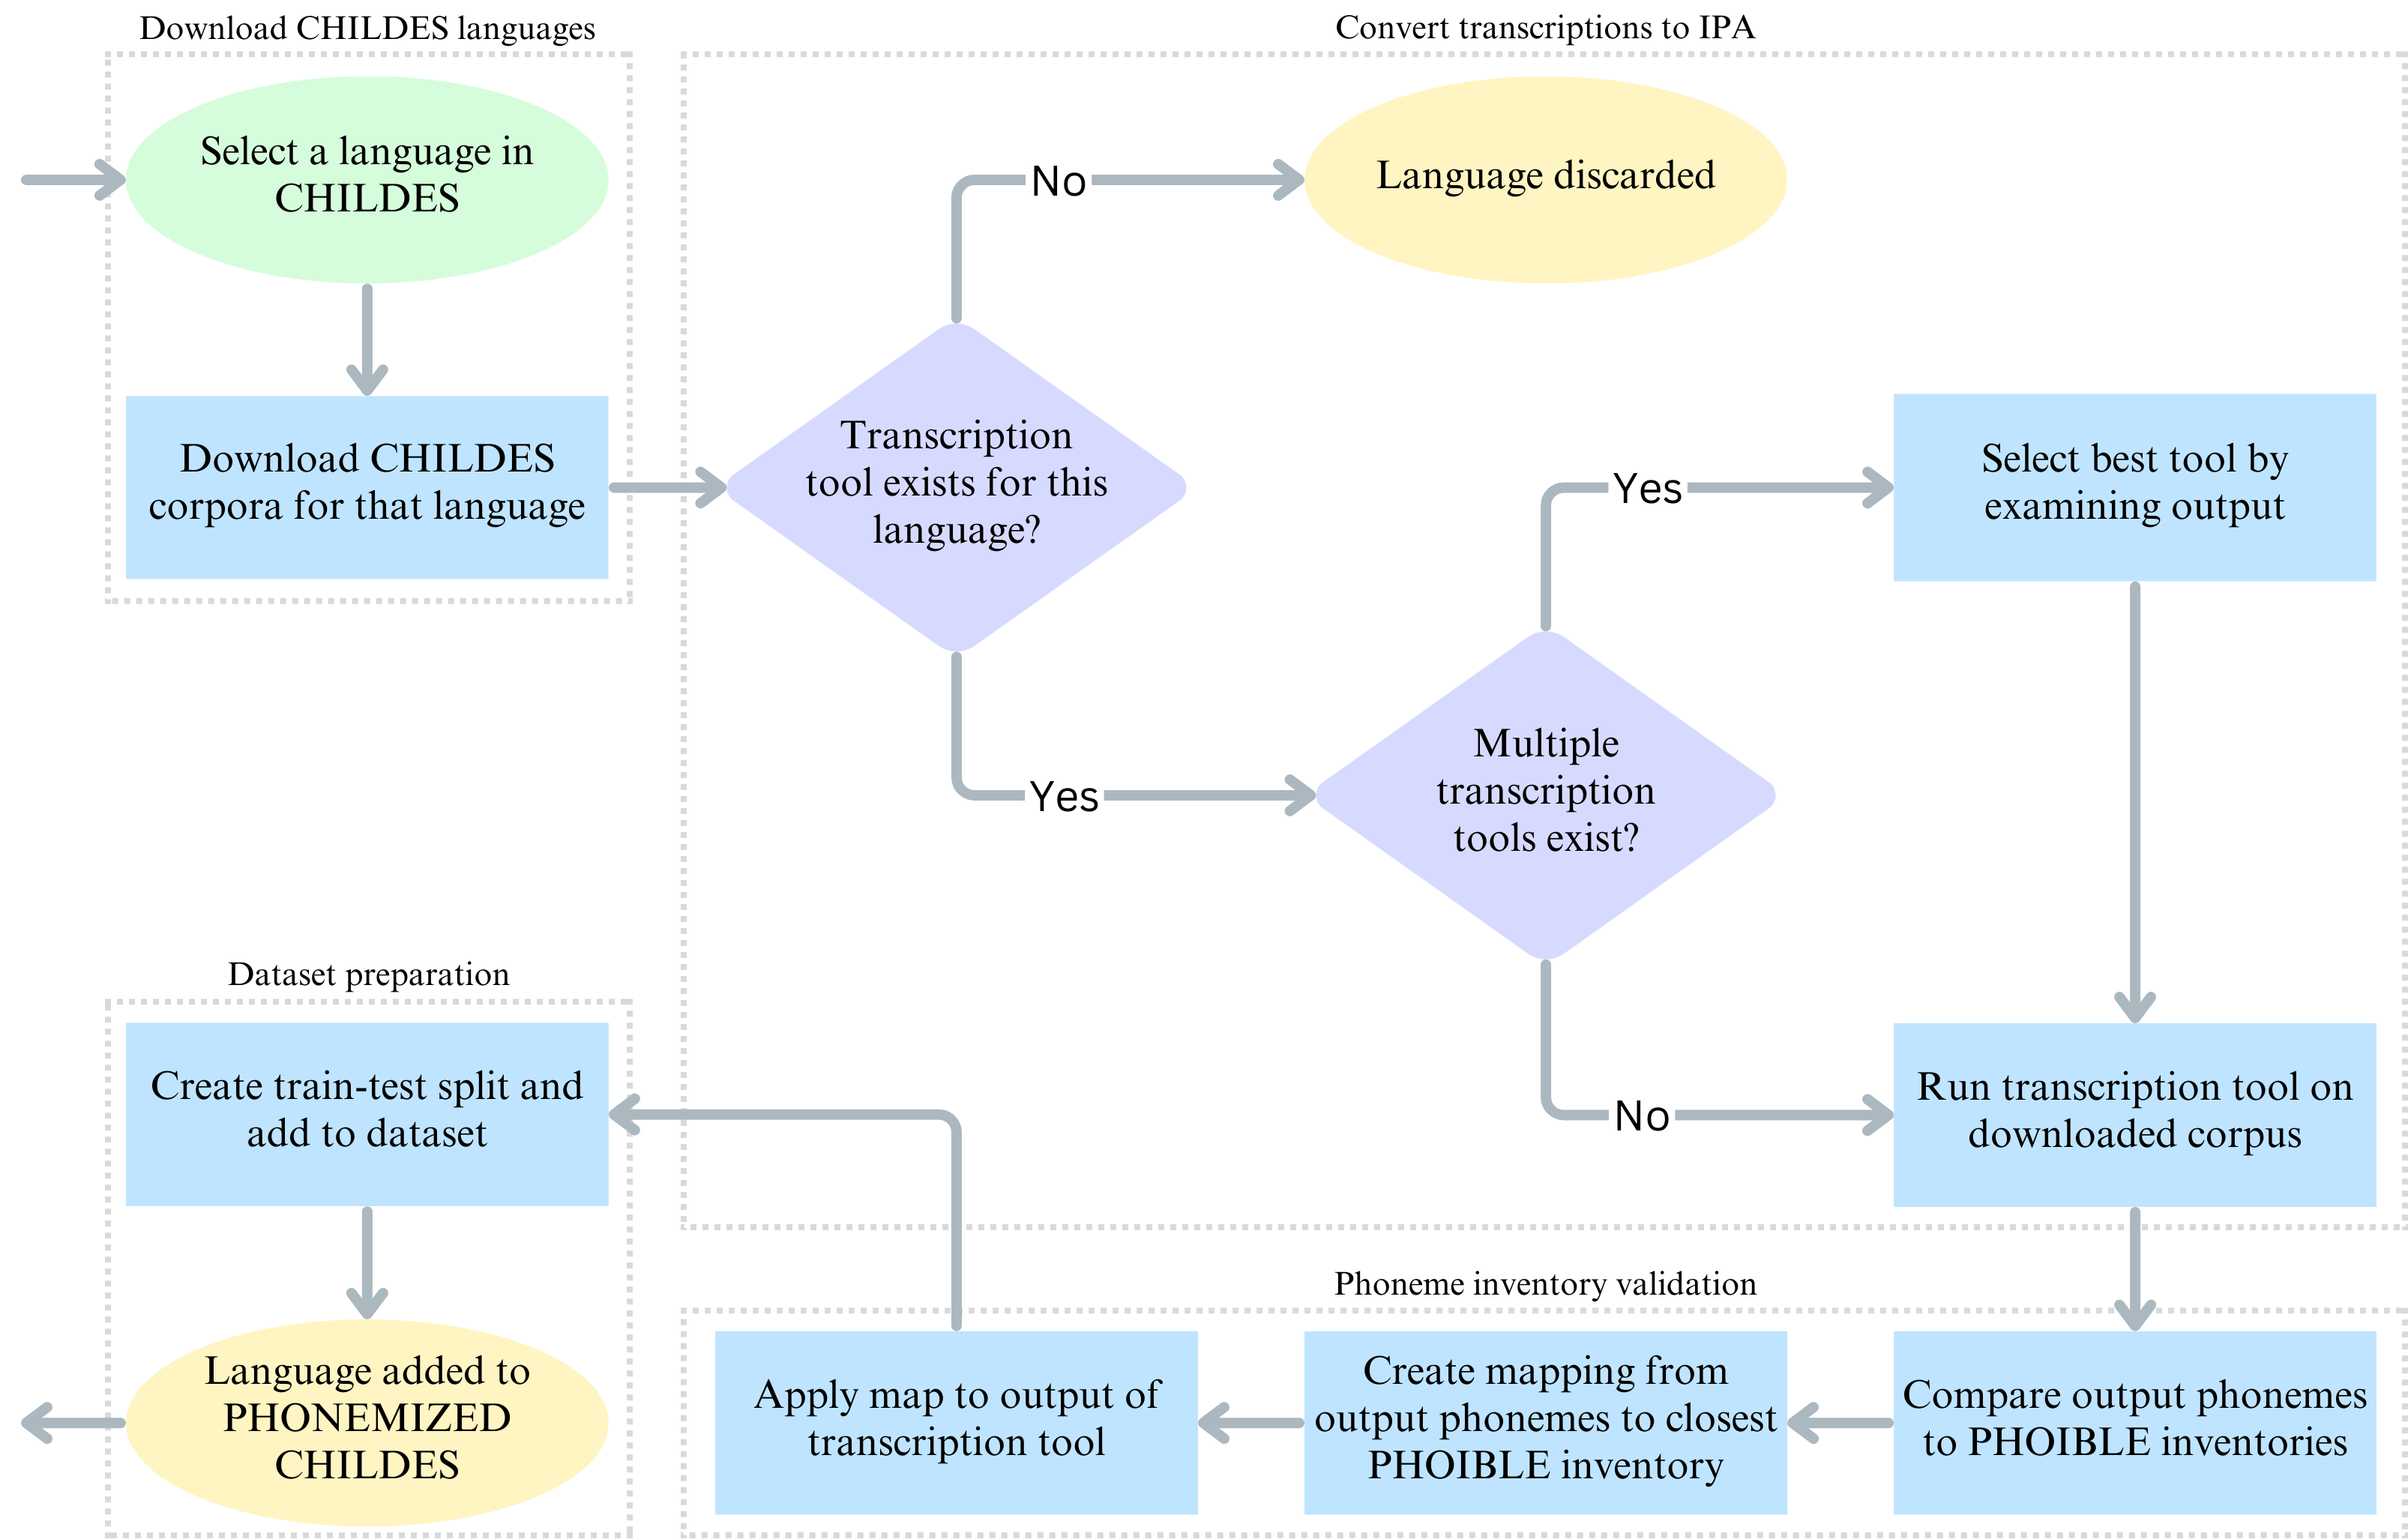
\includegraphics[width=0.9\linewidth]{Figures/13Dataset/data-prep.png}
    \caption{Data preparation pipeline for the Phonemized CHILDES dataset.}
    \label{fig:dataset-data-prep}
\end{figure}

\subsection{CHILDES}

\rough{Describe CHILDES and what languages are in there. Describe what data is available and how we download it.}

\subsection{Dataset creation}

\rough{I add a tool called CHILDES processor to the Corpus Phonemizer suite to specifically help with downloading, phonemizing, and preparing CHILDES corpora into a huggingface dataset. Given the range of languages in CHILDES, I need to determine which backend to use for each. I then need to examine the output and try to map it to a standard inventory set for that language. Finally, I save each language as a section of a Huggingface dataset, each language is a section and has a train-test split.}

\subsection{Dataset overview}

\rough{Describe resulting dataset, give a large table with details, which tool was used, which inventory we map to, etc.}

\section{Corpus Analysis}

\rough{This is where I use the corpus to analyse the phonemic properties of languages. Experiments include:
\begin{itemize}
    \item Information theoretic properties (Zipf's law, Heap's law, ratios, information rate, n-gram perplexities)
    \item Comparing phoneme properties to character properties (hypothesis: information rate more consistent across langugages when looking at phonemes rather than characters)
    \item Child vs adult speech (extract child utterances in CHILDES and compare MLU, word length etc)
    \item Child-directed vs adult-directed speech (compare CHILDES to BNC)
    \item Phoneme clustering (could possibly be moved to chapter 5 - segmentation): looking at phoneme clusters, possibly vowel harmony and other signals for segmentation.
    \item Child errors (could be moved to chapter 6 - past tense formation): looking at errors that children produce.
\end{itemize}
}